\chapter{Z Compensation}

Normally when machining the assumption is made that the material and the machine are perfectly aligned. This is a reasonable assumption when a whole part is being machined, but may not hold true when re-working an existing part. This is particularly true when engraving. An engraving cut may only be 0.1mm deep, and therefore, any inaccuracy in the surface height will cause the engraved cut to change depth (and width) across the part. In some cases this would make the end result look uneven, in some cases (PCBs particularly) part of the cut may not contact the surface at all.

In theory there are two ways of combating this without compensation. Firstly, you could face your support plate so that you know it's true to the machine. This is a good idea anyway. Secondly use more fixings to hold down the work. This may or may not be an option, and is certainly the preferred option if working in brittle materials like acrylic. The problem is that these mechanisms can only remove a certain amount of inaccuracy, and you still have to check them for flatness.

Z compensation takes an already good setup and uses some fairly simple mathematics to correct the cutter height to the surface at better than machine accuracy. The basic theory is that given an arbitrary set of points any three non-colinear points describes a plane, and the z correction for any point $ P(x,y) $ can be calulated based on that plane. This solution is exact for any target point inside three sample points. R-Cam extends this theory to include points outside the sample region by making the assumption that the sampled points are on a flat surface, and therefore the plane created from a triangle on the edge of the sample field is co-incident with the real surface. This is acceptable for most plates, especially where the samples are near the edge and the curvature is low. Using this trick allows accurate chamfering of plate edges.

\section{Surface Sampling}

Assume for a moment that we have a brass plate mounted on a milling machine to be engraved. The plate is reasonably flat. Take an origin point at the center of the plate, and touch off z=0 on the plate surface. This origin is arbitrary.

In order to do z correction, the height of the surface ($ z_s $) at a series of $ x,y $ points must be known. The best way to do this will vary dependant on the milling interface used. With LinuxCNC, we can set up a touch probe and then use the G38.2 command to probe the surface as in the code below which probes 100 points over a 50mm square to a depth of 1mm below the datum. The probe data is stored in probe.txt, which can be given an absolute path to make finding the file easier.

\begin{lstlisting}[caption=Example Probing Code]
(Initialisation)
G21 (Set units to mm)
G90 (Use absolute distances)
G94 (feed in metres/min)
G92.1 (cancel offsets)
G91.1 (incremental arc mode)
G54 (use co-ord system 1)
G98 (set retract behaviour for canned cycles)
G49 (cancel tool length offset)
G40 (cancel cutter compensation)
G17 (select XY plane)
G80 (cancel canned cycle motion mode)

#<_zSafe>=2

#<xMin>=-25
#<yMin>=-25
#<xMax>=25
#<yMax>=25
#<step>=5
#<zMin>=-1

F120

G0 Z#<_zSafe>

#<xFlag>=0

(PROBEOPEN probe.txt)
    
#<x>=#<xMin>
O161 do
  #<y>=#<yMin>
  #<yFlag>=0
  O167 if [#<x> gt #<xMax>]
    #<xFlag>=1
    #<x>=#<xMax>
  O167 endif
  
  O162 do
    O168 if [#<y> gt #<yMax>]
      #<yFlag>=1
      #<y>=#<yMax>
    O168 endif
    G0 X#<x> Y#<y>
    
    G38.2 Z[#<zMin>]
    
    G0 Z#<_zSafe>
    
    #<y>=[#<y>+#<step>]
  O162 while [#<yFlag> eq 0]
  #<x>=[#<x>+#<step>]
O161 while [#<xFlag> eq 0]

(PROBECLOSE)
    
M2
\end{lstlisting}

The code produces a probe file which looks like :

\begin{lstlisting}[caption=Probe file extract]
10.000000 0.000000 -0.108711 0.000000 0.000000 0.000000 ...
10.000000 5.000000 -0.088269 0.000000 0.000000 0.000000 ...
10.000000 10.000000 -0.074009 0.000000 0.000000 0.000000 ...
\end{lstlisting}

The file contains a column for each available axis. R-Cam only uses X,Y,Z axes, thus only the first three columns are of interest. A typical surface sample may look like figure \ref{fig:zComp:probeHeightmap}. Note the change in z across the plate is about 0.4mm across corners. In this case screws were used to hold down the plate and the points probed on the screws have been removed.

\begin{figure}[h]
  \centering
  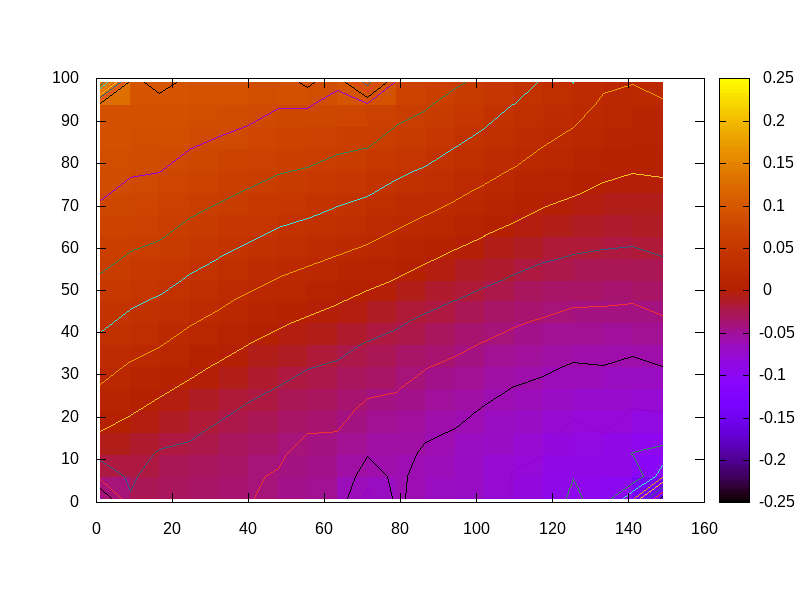
\includegraphics[width=0.7\textwidth]{figures/probeHeightmap.png}
  \caption{Heightmap of a probed plate}
  \label{fig:zComp:probeHeightmap}
\end{figure}

\section{Surface Mathematics}

The definition of a plane may be given in cartesian co-ordinates as

\begin{equation}
ax+by+cz=d
\label{eq:zComp:plane}
\end{equation}

where the vector $\left[ {\begin{array}{c} a \\ b \\ c \end{array}} \right]$ is the normal vector to the plane.

The normal vector to the plane can be found as the cross-product of two non-colinear vectors. The vectors are defined by three points. The point at which we are attempting to machine (the point along the machine path curve) is described as the target point $P(x,y)$. R-Cam takes the closest two points to the target then searches for the next closest point for which the normal vector has a non-zero $z$ value. This ensures that for any target point the most suitable points are used and the offset does not become infinite.

Taking the points as $P_1$, $P_2$ and $P_3$, two vectors are defined as

\begin{eqnarray}
\vec{A}=P_2-P_1 \\
\vec{B}=P_3-P_1
\end{eqnarray}

from which the normal vector is defined as

\begin{equation}
\vec{N}=\vec{A} \times \vec{B}
\end{equation}

The remaining term ($d$)in equation \ref{eq:zComp:plane} is calculated using $P_1$, and the z location of the target point is

\begin{equation}
Z_{P(x,y)}=\frac{d-{N_x}x-{N_y}y}{N_z}
\end{equation}
